\section{Requirements}\label{sec:requirements}
\subsection{Epics}\label{subsec:epics}
Epics were defined at the very beginning of the project and are largely product focussed.
Epics are defined in the Epics section of the Planning tab in Gitlab (\href{https://gitlab.ti.bfh.ch/groups/decibel-threshold-event-displayer/-/epics}{Gitlab}). Epics are subject to change
but for the sake of completeness, they are included in this document anyway (see \autoref{fig:epics}).
\begin{figure}[H]
    \centering
    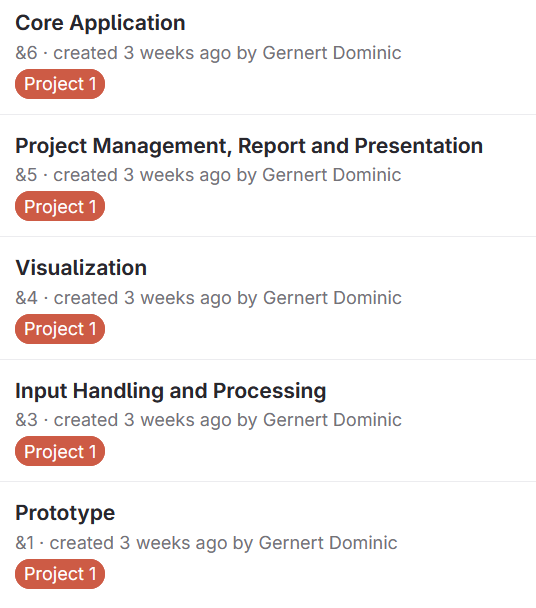
\includegraphics[width=0.5\textwidth]{epics_interim_presentation.png}
    \caption{Epics}\label{fig:epics}
\end{figure}
\subsection{User Stories}\label{subsec:user-stories}
User Stories are created as Issues in Gitlab.
They are associated with an Epic and are prioritised.
Issues contain a \textit{Definition of Ready} (\ref{subsubsec:dor}), Acceptance Criteria, as well as a \textit{Definition of Done} (\ref{subsubsec:dod}).
When an issue is selected for a sprint, sub-tasks are created, estimated and assigned.
The issue itself is assigned to the person with the most assigned sub-tasks.
The full list of issues is available in \href{https://gitlab.ti.bfh.ch/groups/decibel-threshold-event-displayer/-/issues}{Gitlab's issue list} or the \href{https://gitlab.ti.bfh.ch/decibel-threshold-event-displayer/decibel-threshold-event-displayer/-/boards/2832}{Development Board}.

\subsubsection{Definition of Ready}\label{subsubsec:dor}
The \textit{Definition of Ready} is defined as a checklist on every User Story.
In every Sprint Planning the issues selected for
the next Sprint are validated by crossing off the checklist.
All necessary adjustments are made together by the project team before the issue is
estimated and planned.
The \textit{Definition of Ready} is part of the Issue Template in the repository
(see \href{https://gitlab.ti.bfh.ch/decibel-threshold-event-displayer/decibel-threshold-event-displayer/-/blob/main/.gitlab/issue_templates/User\%20Story.md}{Gitlab}). \\ \\
\textit{Definition of Ready}:
\begin{itemize}
    \item Requirements and Acceptance Criteria Defined
    \item Acceptance Criteria must be testable
    \item Understood by the Team
    \item Sized and estimated
    \item Prioritised in the Backlog
    \item No major Impediments
\end{itemize}
\subsubsection{Definition of Done}\label{subsubsec:dod}
Similarly to the \textit{Definition of Ready} (\ref{subsubsec:dor}), the \textit{Definition of Done} is a static checklist that is part of
the issue template.
The tasks are checked off by the reviewer, which is the Product Owner unless specified otherwise. \\ \\
\textit{Definition of Done}:
\begin{itemize}
    \item Acceptance Criteria met
    \item Tested and no critical bugs
    \item Documentation updated
    \item Reviewed and approved
\end{itemize}
\subsection{Product Backlog}\label{subsec:product_backlog}
Issues are prioritised first and foremost by the Product Owner.
This prioritisation is implemented as tags in Gitlab and is can be viewed
on the \href{https://gitlab.ti.bfh.ch/decibel-threshold-event-displayer/decibel-threshold-event-displayer/-/boards/2832}{Development Board} (see\ \autoref{fig:product_backlog})
\begin{figure}[H]
    \centering
    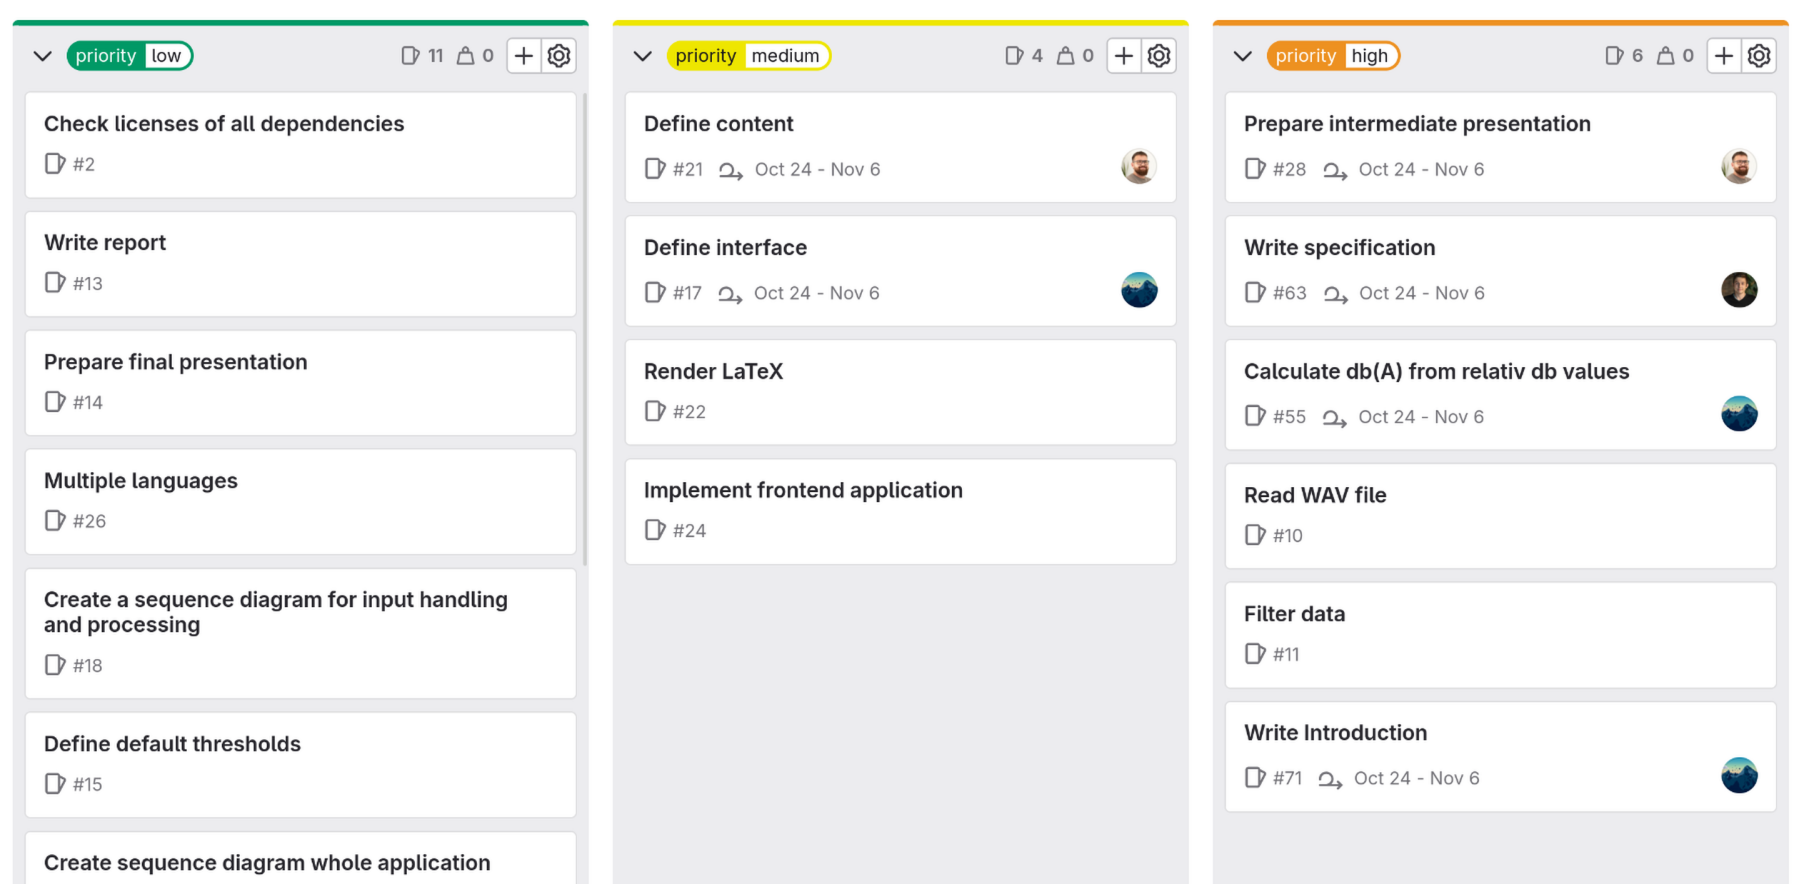
\includegraphics[width=\textwidth]{product_backlog.png}
    \caption{Product Backlog}\label{fig:product_backlog}
\end{figure}
\subsection{Sprint Backlog}\label{subsec:sprint-backlog}
The Sprint Backlog of the currently running sprint is displayed as a column on the \href{https://gitlab.ti.bfh.ch/decibel-threshold-event-displayer/decibel-threshold-event-displayer/-/boards/2832}{Development Board}.
In combination with the prioritisation (see\ \ref{subsec:product_backlog}), this makes for a convenient way for the project team to select issues for the next sprint based on priority (see\ \autoref{fig:sprint_backlog}).
\begin{figure}[H]
    \centering
    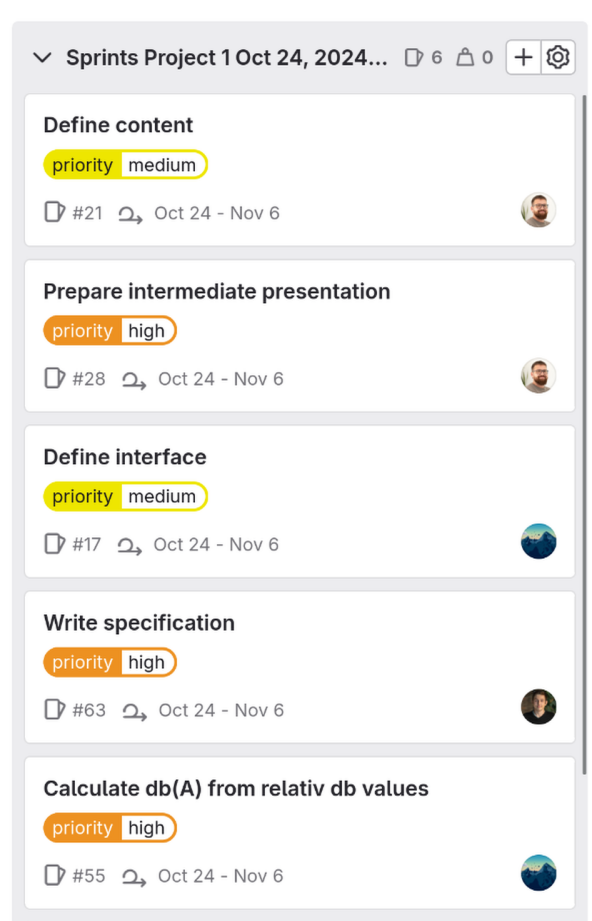
\includegraphics[width=0.5\textwidth]{sprint_backlog_sprint2.png}
    \caption{Sprint Backlog}\label{fig:sprint_backlog}
\end{figure}
\subsection{Impediment Backlog}\label{subsec:impediment_board}
Impediments are also created as Issues in Gitlab.
They are however, assigned the label \textit{Impediment} and are displayed on a separate Impediment Board (see\ \autoref{fig:impediment_board} and \href{https://gitlab.ti.bfh.ch/decibel-threshold-event-displayer/decibel-threshold-event-displayer/-/boards/2834?label_name[]=impediment}{Gitlab}).
Impediments are created either ad hoc or during the Daily Standup meeting.
There is a template for Impediments analogous to the Issue Template (see \href{https://gitlab.ti.bfh.ch/decibel-threshold-event-displayer/decibel-threshold-event-displayer/-/blob/main/.gitlab/issue_templates/Impediment.md}{Gitlab}).
\begin{figure}[H]
    \centering
    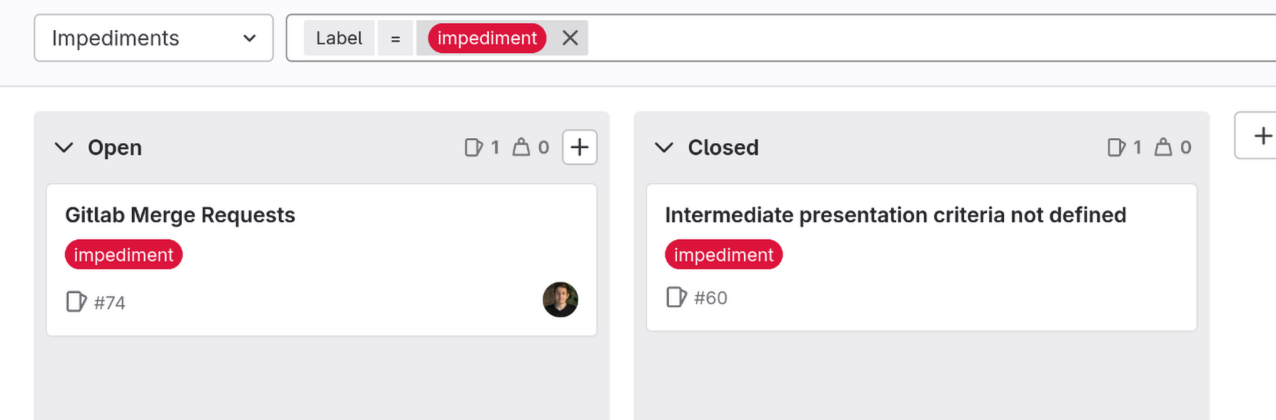
\includegraphics[width=\textwidth]{impediment_board.png}
    \caption{Impediment Board}\label{fig:impediment_board}
\end{figure}